\documentclass[12pt]{article}
\usepackage{cite}
\usepackage{fixltx2e}
\usepackage{graphicx}
\usepackage{float}
\usepackage{array}


\begin{document}
\title{Natural Language to Structured Query Language}



\date{January 15, 2021}
\maketitle



\begin{center}
    
\includegraphics[scale=0.75]{logo}

    \label{fig:Question mark vector}

\end{center}


\centerline{By: Muhammad Usama Alvi (19K-0926)}
\centerline{Supervisor: Dr. Muhammad Rafi}

~\\
~\\

\centerline{National University of Computer and Emerging Sciences}

\newpage




\tableofcontents
\newpage

\listoffigures

\newpage

\listoftables

\newpage


\section{Abstract}
Relational databases are being used world wide to store massive amount of data in numerous fields. However, user faces issues while accessing data from these databases. Users need to understand structured query languages (SQL) in order to query on these databases and fetch results. An average user do not have this knowledge of these query languages. Here NL2SQL tasks play their role for providing an interface to fetch results. These tasks revolves around converting questions written in natural languages to structured query languages using deep learning approaches. This problem has received more attention recently because of large scale dataset releases such as WikiSQL. We have used RoBERTa model to achieve our task. We use RoBERTa model embeddings along with two knwoledge vectors, namely, header knowledge and question knowledge vectors and pass it to LSTM based models to give us final results. We have improved both knowledge vectors which are passed to LSTM based models. The proposed method in the study has been evaluated on WikiSQL dataet. 
\\
\\

\begin{flushleft}
\textbf{General Terms}
\\
Multi-label Classification, Natural language, Structured query language
\\
~\\
\textbf{Keyword and Index Terms}
\\
NL2SQL, SQL, NLP
\end{flushleft}



\newpage

\section{Introduction}
\subsection{Background}
This has been a long standing open problem to provide an interface on which a user, who has no idea about the syntax and working of a structured query language also known as SQL, can write queries in natural language and system converts that natural language to SQL. This SQL executes on database in order to fetch results. Many research has been done on this and still going on in order to bring up the accuracy. Although currently developed models are giving us a accuracy greater than 80\%, there are some dependencies in the model which makes them not suitable to use in practical applications. We will be discussing them as well in related work.
\\ \\
 Relational databases store a vast amount of data and are accessed through structured query languages. Many non technical persons are not familiar with these structured query languages, which creates a lot of trouble and dependencies. If we can remove this structured query language (SQL) dependency, then it would be a lot easier to fetch data from databases. This problem has been given a lot of attention after great number of  large scale datasets has been made available \cite{zhong2017seq2sql} \cite{setlur2019inferencing} \cite{yu2018spider}. 
\\ \\
Pre trained language models such as BERT \cite{devlin2018bert} and RoBERTa \cite{liu2019roberta}  have gained a lot of success in the area of natural language processing tasks. \cite{guo2019content} has done some amazing work using BERT on WikiSQL dataset. It has utilized the pre-trained model BERT as well as database table content in order to achieve state of the art model with highest accuracy. This comes with some limitations which we will discuss in related work. 
\\Although there are number of models having significant accuracies on WikiSQL dataset, accuracies are still limited on Spider benchmark\cite{yu2018spider}. One of the reasons is that Spider dataset is more complex compared to WikiSQL dataset. WikiSQL focuses on rather simpler queries having single or multiple where clauses and no joins.\\\\\\

\subsection{Motivation}
Strcutured query lagnauges has always been a bottleneck for researchers who are not familiar with the ways of structured query langauges. This unfamiliarity creates an additional dependency for researchers in order to interact with databases for the dependency of data. If we are able to make a program, model, some kind of interface which lets researchers or any native users interact with databases without any prior knowledge of database, it will save a lot of time and resources. This has been a primarily source of motivaion to decouple this dependency in order to save time and energy as well. 




\newpage

\section{Related Work}

In this section, we will review the past contributions that has brought natural language to structured query langauge task closer to real world solutions. 

\subsection{Problems with Previous Approaches}

Problem of converting plain text into a structured query language (SQL) is a problem of semantic parsing. It has been wildly in the focus of database communities. In the beginning, focus was more on rule based techniques \cite{setlur2016eviza}, but after the release of large scale databases \cite{yu2018spider} \cite{zhong2017seq2sql}, more approaches has come forward. Recent approaches are now NLP based. Some of the broader categories are - sequence to tree, sequence to sequence and SQL sketch. These approaches comes with their pros and cons. One of the issues of Seq2Seq discussed in \cite{xu2017sqlnet} is that it faces the order matters problem. In order to convert natural language query to
structured query language, we use sequence-to-sequence style model. In order to use this type of model, we have to serialize SQL queries. Here is the problematic part. Since there can be multiple correct queries, it creates different serializations for each query which is not good. Example shown in figure \ref{fig:Order Matters}. There are some approaches which helps overcome this issue. One of the solution for this type of issue is to rely on reinforcement learning to reward the decoder when it comes with any of the correct serializations \cite{xu2017sqlnet}. 


\begin{figure}[H]
    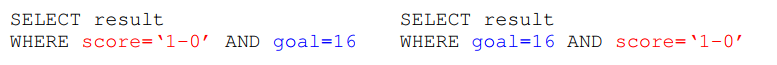
\includegraphics[width=300pt]{OrderMatters}
    \caption{Order Matters}
    \label{fig:Order Matters}
\end{figure}

\subsection{SQLNet}
SQLNet \cite{xu2017sqlnet} works differently from Seq2Seq method. It creates the sketch of important features and then these features are predicted individually as shown in figure \ref{sqlsketch}. It uses column attention method and uses LSTM to encode question and headers. There are number of models which are built on top of this with some variations. For example, SQLova \cite{hwang2019comprehensive} uses the BERT encoders instead of LSTM. 
\\
\\
\\
\begin{figure}[H]
    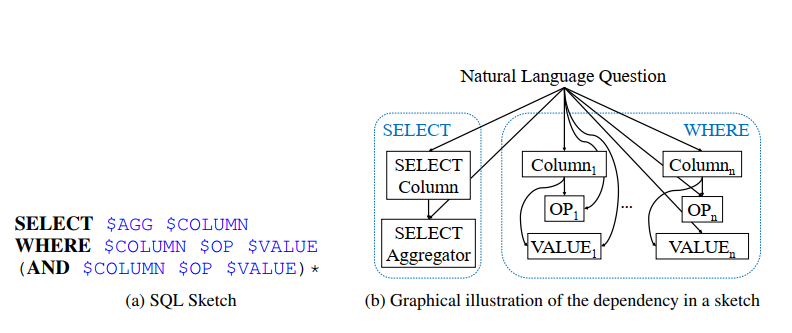
\includegraphics[width=400pt]{sqlsketch}
    \caption{Sketch syntax and the dependency in a sketch}
    \label{sqlsketch}
\end{figure}

\subsection{Content Enhanced Model}
NL2SQL-Rule \cite{guo2019content} uses table content as well while predicting the SQL. It marks vectors to indicate the match of question and headers across two parts and provide it in BERT representations as shown in figure \ref{cellfeature}. However, ColloQL uses table content in BERT encoders. Another technique on top that is used frequently with these models is Execution Guided (EG) decoding. This was first introduced in \cite{wang2018robust}. In this technique, partial SQL queries are executed and their results are used as a guidance for decoding process. However, this is not very helpful in real world. In real world applications, tables have records in millions which would make this process very slow and time consuming. Moreover, EG methods change query on the basis of whether empty result is returned, which is not always due to an erroneous query, but it works on WikiSQL dataset setting. \\
\begin{figure}[H]
    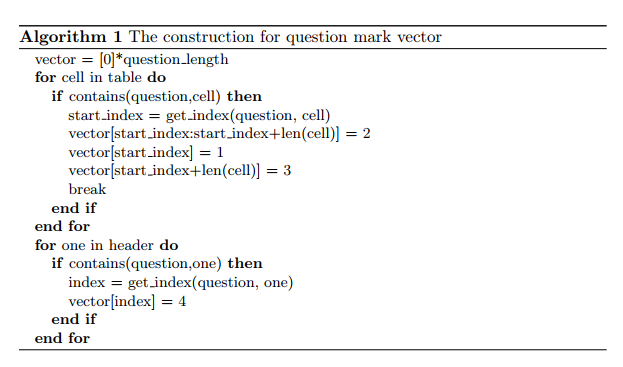
\includegraphics[width=400pt]{cellfeature}
    \caption{Knowledge vector using cell data}
    \label{cellfeature}
\end{figure}
One of the drawbacks using content to enhance your model is the data privacy. When table content and data is provided in the training step, it's privacy is being compromised. There are some industries where data has privacy issues and can not use for the training of model. In order to address this issue, some work has been done. \cite{pal2020data} tried to address this issue using RoBERTa model. It has suggested data agnostic methods. It has eliminated the use of table data and gives the structured query language (SQL) utilizing only table schema and the provided natural language question. Although they were able to completely eliminate table content, there was privacy v/s performance tradeoff. Using this technique, model is capable of zero shot learning and it makes it scalable as well. Headers and natural language question embeddings were created using RoBERTa model and it was provided for prediction along with two knowledge vectors, namely, Question Mark Vector and Header Mark Vector. These are the binary knowledge vectors and important of these vectors are marked with 1 which tells the model the importance and to focus more on this part. It is calculated with the matching tokens across the table schema (Headers) and the natural language question. RoBERTa embedding layer plays an important part of this problem. It is possible that there are very few matches across natural language question and the Headers, therefore, two knowledge vectors will not have useful information. Since RoBERTa is already trained on masked language modeling tasks and they have the sense of knowledge and context, it can be very helpful in solving the above problem. \\
\subsection{IRNet}
IRNet is one of the known effective model for this problem \cite{guo2019towards}. It is used for complex and cross-domain text to structured query language. The main focus of this model has been on two issues. First is to address the mismatch between the queries written in natural language and the generated SQL. Second is to increase the accuracy in generating the column for SQL. Generating the column for SQL has been difficult due to the use of out of domain words. 
\subsection{X-SQL}
Another approach that is used is called X-SQL. It is a new network architecture. X-SQL proposes to reinforce the contextual output from BERT-style pre training model into the structural schema representation, and learn a new schema representation for downstream tasks. This is tested on WikiSQL data set and it shows better results than the state of the art models. Results were improved on development as well as test sets \cite{bogin2019global}.






\section{Research Methodology}
\subsection{Dataset}
WikiSQL is a large semantic parsing dataset. It contains around 24,241 tables and 80,654 natural language questions and it has corresponding structured query languages to those questions. Releasing this dataset has brought much attention to NLP2SQL task. Having this big dataset, it has enabled deep neural techniques to adopt this task. However, it contains simpler queries which do not have any joins and have at most one relation. 
\begin{figure}[H]
    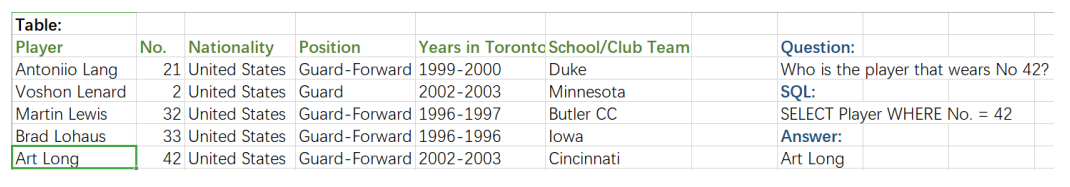
\includegraphics[width=450pt]{wikisql}
	\caption{An example of WikiSQL dataset}
    \label{fig:WikiSQL}
\end{figure}


\subsection{Implementation}
We have implemented two based models based on BERT and RoBERTa, in order to build up our implementation on top of it. In the following section, we will be going through each implementation and their differences along with advantages and disadvantages. 

\subsection{RoBERTa}
In RoBERTa based model, we generate two knowledge vectors to give our model more confidence. These two are binary vectors and tell model which part are more important and need to be focused on by marking that specific parts. They encode the significance of headers and question tokens. Both of these vectors are then concatenated together and passed as additional features to model in order to bring more confidence in models. 


\subsubsection{Question Mark Vector}
\begin{figure}[H]
    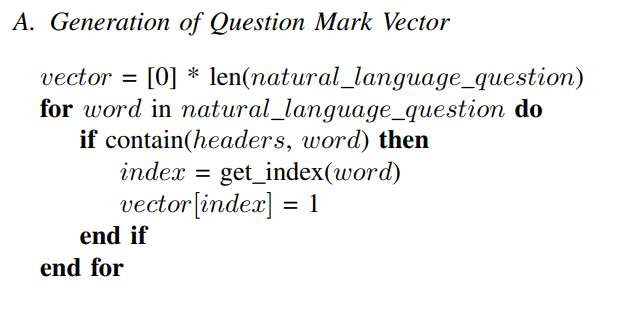
\includegraphics[width=300pt]{QMV}
    \caption{Question Mark Vector}
    \label{fig:Question mark vector}
\end{figure}

First, vector is initialized of same length as natural language question and assigned all the zeros in Fig 2. After initialization, program loops on natural language question tokens. Headers and each token of natural language question is passed in "contains" function which returns true if the token exists in headers, and false if it does not exist. If the token exists in header, then token index position is marked in vector with 1, otherwise, value remains 0 as per initialization. 


\subsubsection{Header Mark Vector}
\begin{figure}[H]
    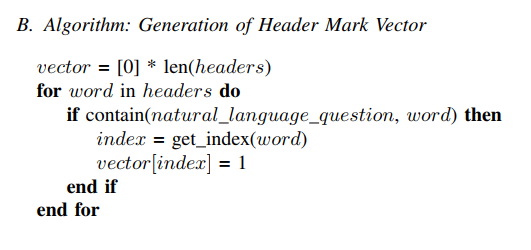
\includegraphics[width=300pt]{HMV}
    \caption{Header Mark Vector}
    \label{fig:Header mark vector}
\end{figure}

For header mark vector, we follow same procedure. Frist, vector is initialized of same length as headers and assigned all the values to zero in Fig 3. After initialization, program loops on headers. Each header and natural language question is passed in "contains" function which returns true if the header exists in questions, and false if it does not exist. If the header exists in question, then header index position is marked in vector with 1, otherwise, value remains 0 as per initialization. One thing to notice here is that loop iteration is not over headers here, rather it is on individual words in headers. Moreover, one thing that is majorly different here from \cite{guo2019content} is that we do not iterate through data here, hence maintaining the data integrity and privacy.


\subsection{BERT}
In BERT based model, we generate two knowledge vectors as well to give our model more confidence. These two are binary vectors same as in the case of RoBERTa and tell model which part are more important and need to be focused on by marking that specific parts. They encode the significance of headers and question tokens. Both of these vectors are then concatenated together and passed as additional features to model in order to bring more confidence in models. The main difference comes in the encoding. Here we encode based on the actual data which compromises the privacy of the data. Here we need the actual data for the encoding and for the elarning phase of the model. 

\subsubsection{Question Mark Vector}
For the encoding of Question amrk vector, we crete a vector of question's length initialized with zeros only. After initialization, we iterate through each cell in table data and if there is a match between cell data and question, then respective position of question vector is marked. One important thing to note here is that we are iterating through table data as hown in figure \ref{cellfeature1}. This compromises the privacy of data. Although this increases the accuracy of the model due to training ona ctual data, it exposes actual data to model. 

\begin{figure}[H]
    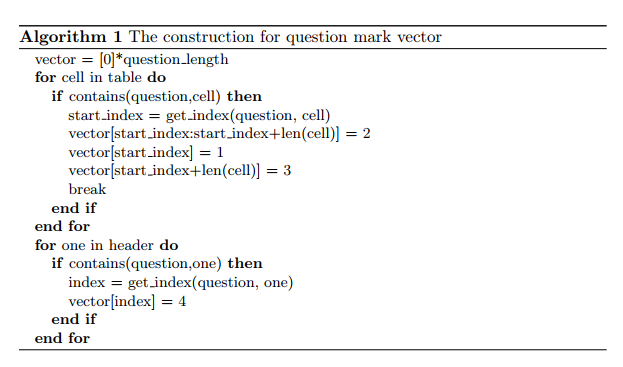
\includegraphics[width=400pt]{cellfeature}
    \caption{Knowledge vector using cell data}
    \label{cellfeature1}
\end{figure}

\subsubsection{Header Mark Vector}
For this vector, we initialize vector with zeros of ehader length. We iterate though cell data as well for marking positions of great importance which can convey useful information to the model. Once again, this vector as well compromises the privacy of actual data while training. 

\begin{figure}[H]
    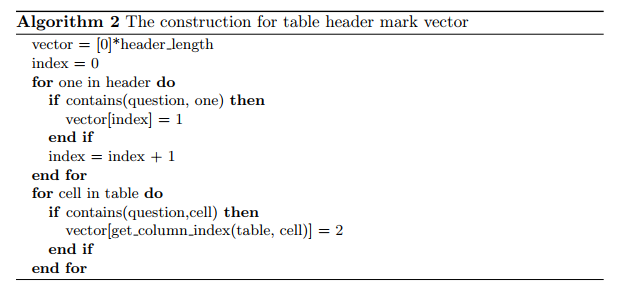
\includegraphics[width=400pt]{headermarkvetorbert}
    \caption{Header vector using cell data}
    \label{headermarkvetorbert1}
\end{figure}


\subsection{Model}
Sequence to sequence style model is not recommended to use here because of the "order-matters" problem. It is possible for SQL query to have more than one correct queries. It is possible to move some conditions ordering and still get correct result. However, sequence to sequence style model choses one ordering correct and it labels other queries as wrong. In order to overcome this issue, another approach is used here suggested by SQLNet \cite{xu2017sqlnet}. It uses sketch based approach to predict SQL queries. However, unlike sequence to sequence, it eliminates the task of predicting complete queries and reduced that task into predicting some parts of it only. Hence the order matters problem is eliminated here. SQL query sketch:
 
\begin{figure}[H]
    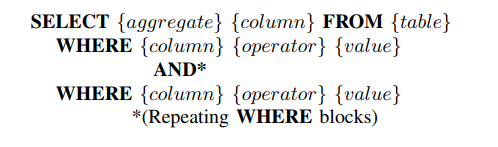
\includegraphics[width=300pt]{sketch}
    \caption{Query Sketch}
    \label{fig:Query Sketch}
\end{figure}

In fig 3, we can see all the parts which will be filled by models predictions instead of complete queries. 
\\
\\
Natural language question along with table headers is given input to RoBERTa model. It gives us embeddings which are then used for downstream tasks.  These embeddings along with the concatenation of question mark vector and header mark vector is passed into sub models in order to predict and fill SQL sketch. Model architecture is shown in Fig 5. 

\begin{figure}[H]
    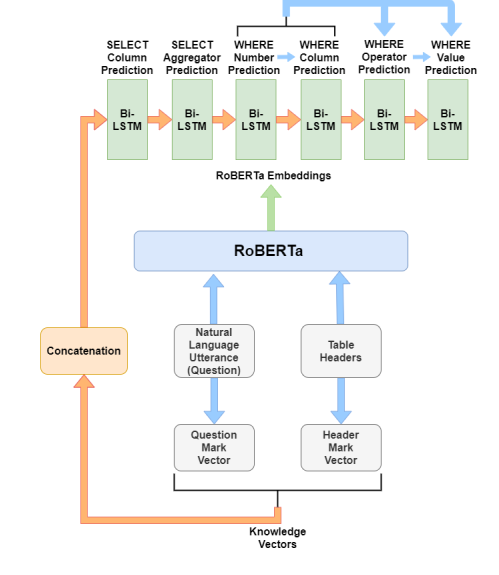
\includegraphics[width=350pt]{model}
    \caption{Model Architecture}
    \label{fig:Model Architecture}
\end{figure}

Embedding layer in this architecture plays an important role. Since we pass two knowledge vectors as well along with RoBERTa embedding into sub models for downstream tasks, it is important to not make our model depend on these two knowledge vectors completely. It is because there is a possibility that natural language question does not match with headers token, hence, not giving much information. If there are no matches between natural language questions and header tokens, then vectors would be consisting of zeros and would not give much information to model. Therefore, embeddings is very important and that is why RoBERTa embeddings is used here. 
\\
\\
It is important for model to extract significance amount of information from natural language question and table headers. Hence, both of these information is passed in RoBERTa model as shown in Fig 4. Similar architecture is used in \cite{guo2019content}, but vectors are generated using table content, hence, compromising data privacy. Another reason to use RoBERTa model is to have some sense of knowledge and context in model so that it can understand the meaning is same of even mismatched tokens. RoBERTa is pre trained on very large corpus of 160 GB and on masked language modeling, next sentence predictions tasks. This gives the model desired sense of knowledge and context. 


\section{Reproducing State of the Art}

We have implemented two state of the art models \cite{guo2019content}, \cite{liu2019roberta}, giving us the inside of core implementations. \cite{guo2019content} is the basic model and \cite{liu2019roberta} is built on top of this model. Therefore, understanding these two implementations and their differences is very important. 

\subsection{BERT and RoBERTa Model}

BERT and RoBERTa are pre trained model on a very large corpus about 16 GB and 160 GB data respectively. They are trained on masked language modeling task and next sentence prediction task as well. This training on large corpus gives them the sense of "knowledge" and "context". \cite{guo2019content} uses two knowledge vectors as well explained in fig. 2 and fig. 3. However, the major difference comes in Question Mark Vector. In \cite{guo2019content}, loop goes through the cell values where as in  \cite{pal2020data} goes through header tokens, hence respecting the data privacy. This is why we have seen  \cite{pal2020data} model has privacy v/s performance trade off.  \cite{pal2020data} has less accuracy compared to \cite{guo2019content}. However, \cite{pal2020data} model does not need data for training, hence, it has zero shot learning. 
\\
\\
After training model we were able to generate similar results as mentioned in paper \cite{pal2020data}. Below is an screenshot of inferring query from natural language question after training the model. 


\begin{figure}[H]
    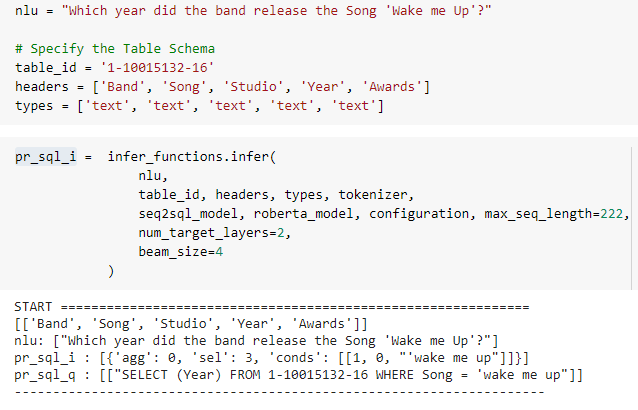
\includegraphics[width=400pt]{infer}
    \caption{Infering Query}
    \label{fig:Infering Query}
\end{figure}


\section{Our Experiment}
We have built our experiment on top of the RoBERTa model. 

\subsection{WordNet}
The WordNet database contains many sorts of relationships between words which help us understand relations between different words. It can categorize words into different hierarchies and answer many interesting questions. If we have a single word "run" and we would like to understand its relations between different words which are in close proximity to it. WordNet can gives us diagram shown in figure \ref{wordnet}.


\begin{figure}[H]
    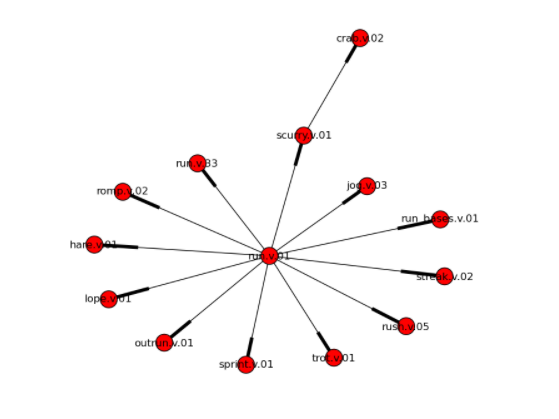
\includegraphics[width=400pt]{wordnet}
    \caption{WordNet}
    \label{wordnet}
\end{figure}

\subsection{Implementation}
We have taken help of WordNet in creating of our two knowledge vectors, header knowledge vector, question knowledge vector. While marking these vectors in order to provide useful information to model with the areas where to focus on, we used to look for exact matches in the headers and questions. Through this method, our vectors were loosing much information which cold help model gain some accuracy and show better results. In our implementation, we did not look for exact amtches, rather, we created two synsets and calculated the probability of their match. We marked vectors if the probability was greater than or equal to 0.7. 

\subsubsection{why?}
It is quite common in natural language that we sometimes use synchronyms in our sentences and not exact words which were affecting results in our problem domain. Not only synchronyms, but the use of singualr words and plural words were also affecting our model, since, singular and plural does not result in exact match as well. 

\section{Analysis and Results}


We have evaluated our model on the WikiSQL dataset with
the logical form and execution accuracy metrics. The method
of calculating the execution accuracy does involve the model
querying the database which goes against our core objective of
data privacy, but this is not a necessary step and neither does
it affect the model’s training in any way. The only purpose of
such querying is to obtain an additional evaluation metric to
better understand our model’s performance. The final model
when deployed would not need to calculate any such metrics,
thus keeping the data completely private.
We have compared our model with the state of the art model
as well as the baseline SQLNet Model:
Note: Accuracy has been shortened to acc. and execution
has been shortened to exec.

\subsection{BERT with Content Enhanced Implementation}

BERT model implementation with table data included in training gives promising results. However, it compromises the privacy of the data. This implementation is carried out with traditional two knowledge vectors without the additional input of WordNet, results are shown in table \ref{berttable} and table \ref{berttabledetailed}.


 \begin{table}
\centering
 \begin{tabular}{| m{2cm} | m{2cm}| m{2cm} |m{2cm}| m{2cm} |} 
 \hline
Model & Dev logical form acc. & Dev exec acc. & Test logical form acc. & Test exec acc. \\ 
 \hline\hline
  BERT & 84.3\% & 90.3\% & 83.7\% & 89.2\% \\ 
 \hline
\end{tabular}
\caption{Overall result of BERT Model on WikiSQL task}
\label{berttable}
\end{table}

\begin{table}
\centering
 \begin{tabular}{| m{2cm} | m{2cm}| m{2cm} |m{2cm}| m{2cm} |m{2cm} | m{2cm} |} 
 \hline
 Model  & SELECT column & SELECT agg & WHERE number & WHERE column & WHERE op & WHERE value\\ 
 \hline\hline
 BERT & 97.4\% & 90.0\% & 99.1\% & 97.9\% & 98.1\% &  97.6\% \\ 
 \hline

\end{tabular}
\caption{Break down result of BERT model on WikiSQL task}
\label{berttabledetailed}
\end{table}


\subsection{RoBERTa with Traditional Knowledge Vectors}

We implementented RoBERTa model without using table data. It did ensure the privacy of data, however, it did come with its trade off. We marked two knowledge vectors using only headers and natual langauge question. In this model, we did not use any real data for training of the model, rather, we used only schema information of the table. Results are shown in table \ref{robertatable} and table \ref{robertatabledetailed}.

 \begin{table}
\centering
 \begin{tabular}{| m{2cm} | m{2cm}| m{2cm} |m{2cm}| m{2cm} |} 
 \hline
Model & Dev logical form acc. & Dev exec acc. & Test logical form acc. & Test exec acc. \\ 
 \hline\hline
  RoBERTa & 74.4\% & 80.9\% & 73.3\% & 80.3\% \\ 
 \hline
\end{tabular}
\caption{Overall result of RoBERTa Model on WikiSQL task}
\label{robertatable}
\end{table}


\begin{table}
\centering
 \begin{tabular}{| m{2cm} | m{2cm}| m{2cm} |m{2cm}| m{2cm} |m{2cm} | m{2cm} |m{2cm} |} 
 \hline
  Dataset & SELECT column & SELECT agg & WHERE number & WHERE column & WHERE op & WHERE value\\ 
 \hline\hline
  Dev & 96.2\% & 90.6\% & 98.0\% & 91.3\% & 93.4\% &  90.5\% \\ 
\hline
 Test & 95.8\% & 90.4\% & 97.2\% & 89.8\% & 92.4\% &  89.7\% \\ 
 \hline

\end{tabular}
\caption{Break down result of RoBERTa model on WikiSQL task}
\label{robertatabledetailed}
\end{table}

\subsection{RoBERTa Model with Header Knowledge Vector with WordNet}

We implementented RoBERTa model without using table data. We marked two knowledge vectors using only headers and natual langauge question. However, the main difference here is how we did the  encoding of Header knwoledge vector. We encoded vector here with the help of WordNet as explained in Section 6. Results are shown in table \ref{robertatableoneheader} and table \ref{robertatabledetailedoneheader}.



 \begin{table}
\centering
 \begin{tabular}{| m{2cm} | m{2cm}| m{2cm} |m{2cm}| m{2cm} |} 
 \hline
Model & Dev logical form acc. & Dev exec acc. & Test logical form acc. & Test exec acc. \\ 
 \hline\hline
  RoBERTa & 81.0\% & 86.0\% & 80.4\% & 85.4\% \\ 
 \hline
\end{tabular}
\caption{Overall result of RoBERTa Model on WikiSQL task with WordNet Header vector}
\label{robertatableoneheader}
\end{table}


\begin{table}
\centering
 \begin{tabular}{| m{2cm} | m{2cm}| m{2cm} |m{2cm}| m{2cm} |m{2cm} | m{2cm} |m{2cm} |} 
 \hline
  Dataset & SELECT column & SELECT agg & WHERE number & WHERE column & WHERE op & WHERE value\\ 
 \hline\hline
  Dev & 97.0\% & 90.8\% & 98.8\% & 93.8\% & 97.7\% &  95.6\% \\ 
\hline
 Test & 96.8\% & 90.6\% & 98.3\% & 93.3\% & 97.2\% &  95.2\% \\ 
 \hline

\end{tabular}
\caption{Break down result of RoBERTa model on WikiSQL task with WordNet Header vector}
\label{robertatabledetailedoneheader}
\end{table}


\subsection{RoBERTa Model with Question \& Header Knowledge Vectors with WordNet}

We implementented RoBERTa model without using table data. We marked two knowledge vectors using only headers and natual langauge question. However, the main difference here is how we did the  encoding of Header knwoledge vector as well as Question knowledge vector. We encoded vectors here with the help of WordNet as explained in Section 6. Results are shown in table \ref{robertatabletwoheader} and table \ref{robertatabledetailedtwoheader}.

 \begin{table}
\centering
 \begin{tabular}{| m{2cm} | m{2cm}| m{2cm} |m{2cm}| m{2cm} |} 
 \hline
Model & Dev logical form acc. & Dev exec acc. & Test logical form acc. & Test exec acc. \\ 
 \hline\hline
  RoBERTa & 81.4\% & 86.6\% & 80.5\% & 85.8\% \\ 
 \hline
\end{tabular}
\caption{Overall result of RoBERTa Model on WikiSQL task with WordNet knowledge vectors}
\label{robertatabletwoheader}
\end{table}


\begin{table}
\centering
 \begin{tabular}{| m{2cm} | m{2cm}| m{2cm} |m{2cm}| m{2cm} |m{2cm} | m{2cm} |m{2cm} |} 
 \hline
  Dataset & SELECT column & SELECT agg & WHERE number & WHERE column & WHERE op & WHERE value\\ 
 \hline\hline
  Dev & 97.2\% & 90.8\% & 98.8\% & 94.0\% & 97.9\% &  95.9\% \\ 
\hline
 Test & 96.7\% & 90.7\% & 98.3\% & 93.4\% & 97.3\% &  95.3\% \\ 
 \hline

\end{tabular}
\caption{Break down result of RoBERTa model on WikiSQL task with WordNet knowledge vectors}
\label{robertatabledetailedtwoheader}
\end{table}



\section{Conclusion}
In this experiment, the focus was on building the model without using the data available in database due to obvious privacy issues. This is a data agnostic model. We have seen that existing models use table content as well as a feature when inputting the model. Moreover, if some models are not using the real data, they make use of execution guided decoding. We have not used any of these two techniques. We have developed a data blind model using only table schema. 
\\
\\
Our result table shows that model has achieved 77.0\% accuracy on train set, and 76.7\% on test set. This is using WikiSQL dataset. This is a highly generalized model since any part of real data was not used. 

\bibliography{references}
\bibliographystyle{ieeetr}
\end{document}